\chapter*{LAMPIRAN}

\section{Daftar Smart Contract Lakomi}

Keempat \textit{smart contract} Lakomi diimplementasikan menggunakan Solidity 0.8.20 dan di-deploy pada jaringan DChain (Chain ID 17845). Kode sumber lengkap tersedia pada repositori GitHub \url{https://github.com/iZcy/Lakomi}. Tabel \ref{tab:contract-list} merangkum informasi setiap kontrak.

\begin{table}[h]
\centering
\caption{Daftar \textit{Smart Contract} Lakomi}
\label{tab:contract-list}
\footnotesize
\begin{tabular}{p{0.12\textwidth}p{0.08\textwidth}p{0.14\textwidth}p{0.24\textwidth}p{0.30\textwidth}}
\toprule
\textbf{Nama Kontrak} & \textbf{Lines of Code} & \textbf{Inherits} & \textbf{Roles} & \textbf{Fungsi Utama} \\
\midrule
LakomiToken & \textasciitilde 230 & ERC20, AccessControl, Reentrant & ADMIN, MEMBER, MINTER, BURNER, LOCKER & registerMember, resignMember, revokeMember, lockTokens \\
\midrule
LakomiVault & \textasciitilde 410 & AccessControl, Reentrant, Pausable & ADMIN, TREASURER, GOVERN, PENGAWAS, LOAN & payPokok, payWajib, deposit, distributeSHU, claimSHU, getPengawasAudit \\
\midrule
LakomiGovern & \textasciitilde 280 & AccessControl, Reentrant, Pausable & ADMIN, PENGAWAS, GOVERN & createProposal, castVote, execute, veto, beginElection, finalizeElection, scheduleRAT \\
\midrule
LakomiLoans & \textasciitilde 270 & AccessControl, Reentrant, Pausable & ADMIN, APPROVER & requestLoan, approveLoan, disburse, repay, markDefault, claimCollateral \\
\bottomrule
\end{tabular}
\end{table}

\section{Struktur Data Utama}

Setiap \textit{smart contract} mendefinisikan struktur data yang memetakan ketentuan UU 25/1992. Berikut adalah definisi \texttt{struct} dan \texttt{enum} utama yang digunakan dalam sistem.

\subsection{LakomiToken --- Keanggotaan}

\begin{lstlisting}
enum MemberStatus { None, Active, Suspended, Resigned, Revoked }
enum ContributionTier { None, Basic, Silver, Gold }

struct MemberInfo {
    MemberStatus status;
    ContributionTier tier;
    uint256 joinedAt;
    uint256 resignedAt;
    uint256 cumulativeSimpanan;
    uint256 lockedCollateral;
    uint256 outstandingLoans;
}
\end{lstlisting}

\subsection{LakomiVault --- Simpanan dan SHU}

\begin{lstlisting}
enum SHUCategory {
    Cadangan, JasaModal, JasaUsaha, 
    Pendidikan, Pengurus, KesejahteraanSosial
}

struct Distribution {
    uint256 totalAmount;
    uint256 sharesTotal;
    uint256 timestamp;
    mapping(SHUCategory => uint256) categoryAmounts;
    mapping(address => bool) claimed;
}

struct PendingWithdrawal {
    uint256 amount;
    uint256 requestTime;
    uint256 approvalCount;
    bool approved;
}
\end{lstlisting}

\subsection{LakomiGovern --- Proposal dan Pemilihan}

\begin{lstlisting}
enum ProposalType { 
    SPEND, PARAMETER, MEMBERSHIP, RAT_ANNUAL, CUSTOM 
}
enum ProposalStatus { 
    Created, Active, Succeeded, Defeated, 
    Queued, Executed, Vetoed, Canceled 
}

struct Proposal {
    address proposer;
    string title;
    string description;
    ProposalType pType;
    bytes data;
    ProposalStatus status;
    uint256 startBlock;
    uint256 endBlock;
    uint256 forVotes;
    uint256 againstVotes;
    uint256 abstainVotes;
    mapping(address => bool) hasVoted;
    bool vetoed;
    bool executed;
}

struct Election {
    bytes32 role;
    mapping(address => bool) candidates;
    mapping(address => uint256) votes;
    mapping(address => bool) hasVoted;
    uint256 startTime;
    uint256 endTime;
    uint256 termLength;
    bool finalized;
    address winner;
}
\end{lstlisting}

\subsection{LakomiLoans --- Pinjaman}

\begin{lstlisting}
enum LoanStatus { 
    Pending, Approved, Active, Repaid, 
    Defaulted, CollateralClaimed 
}

struct Loan {
    address borrower;
    uint256 principal;
    uint256 interestRate;
    uint256 duration;
    uint256 collateralAmount;
    uint256 disbursedAt;
    uint256 repaidAmount;
    uint256 lastPaymentAt;
    LoanStatus status;
    address approvedBy;
    bool collateralLocked;
}

struct BorrowerInfo {
    uint256 activeLoanCount;
    uint256 totalBorrowed;
    uint256 totalRepaid;
    uint256 defaultCount;
    uint256 lastLoanAt;
}
\end{lstlisting}

\section{Diagram Alur Transaksi}

Gambar \ref{fig:transaction-flow} mengilustrasikan alur transaksi lengkap dalam sistem Lakomi, dari pendaftaran anggota hingga distribusi SHU.

\begin{figure}[h]
\centering
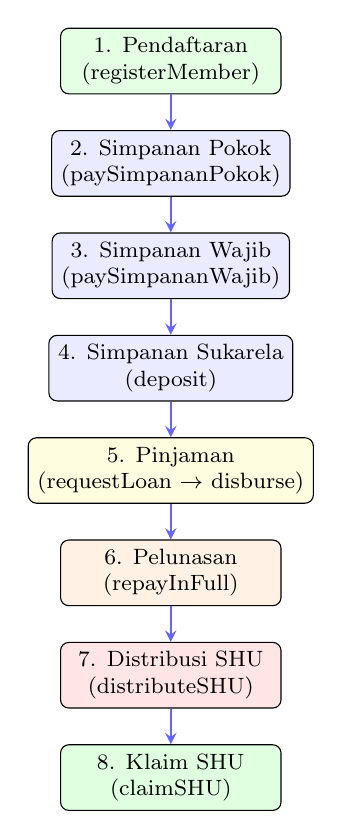
\begin{tikzpicture}[
    node distance=1.0cm,
    box/.style={rectangle, draw, rounded corners=3pt, minimum width=2.8cm, minimum height=0.4cm, font=\footnotesize, align=center},
    arr/.style={->, >=stealth, thick, blue!60},
]
\node[box, fill=green!10] (reg) at (0,5.5) {1. Pendaftaran\\(registerMember)};
\node[box, fill=blue!8] (pokok) at (0,4.2) {2. Simpanan Pokok\\(paySimpananPokok)};
\node[box, fill=blue!8] (wajib) at (0,2.9) {3. Simpanan Wajib\\(paySimpananWajib)};
\node[box, fill=blue!8] (sukarela) at (0,1.6) {4. Simpanan Sukarela\\(deposit)};
\node[box, fill=yellow!12] (loan) at (0,0.3) {5. Pinjaman\\(requestLoan $\to$ disburse)};
\node[box, fill=orange!10] (repay) at (0,-1.0) {6. Pelunasan\\(repayInFull)};
\node[box, fill=red!10] (shu) at (0,-2.3) {7. Distribusi SHU\\(distributeSHU)};
\node[box, fill=green!12] (claim) at (0,-3.6) {8. Klaim SHU\\(claimSHU)};
\draw[arr] (reg) -- (pokok);
\draw[arr] (pokok) -- (wajib);
\draw[arr] (wajib) -- (sukarela);
\draw[arr] (sukarela) -- (loan);
\draw[arr] (loan) -- (repay);
\draw[arr] (repay) -- (shu);
\draw[arr] (shu) -- (claim);
\end{tikzpicture}
\caption{Alur Transaksi Utama dalam Sistem Lakomi}
\label{fig:transaction-flow}
\end{figure}

Siklus dimulai dengan pendaftaran anggota (langkah 1) yang mensyaratkan pembayaran Simpanan Pokok (langkah 2) dan pencetakan 100 token LAK. Anggota kemudian dapat membayar Simpanan Wajib secara periodik (langkah 3) dan menyetor Simpanan Sukarela (langkah 4). Setelah memiliki \textit{tier} kontribusi, anggota dapat mengajukan pinjaman (langkah 5) melalui proses persetujuan dan pencairan. Pelunasan pinjaman (langkah 6) mengalirkan bunga ke LakomiVault sebagai pendapatan. Secara periodik, GOVERN\_ROLE mendistribusikan SHU (langkah 7) dari akumulasi pendapatan ke enam kategori. Anggota kemudian mengklaim SHU masing-masing (langkah 8) berdasarkan \textit{shares}.

\section{Konfigurasi Role-Based Access Control}

Tabel \ref{tab:role-matrix} menyajikan matriks akses berbasis peran (\textit{role-based access matrix}) yang menunjukkan fungsi-fungsi mana yang dapat diakses oleh setiap peran. Simbol $\checkmark$ menunjukkan akses diizinkan, $\times$ menunjukkan akses ditolak.

\begin{table}[h]
\centering
\caption{Matriks Akses Berbasis Peran pada Sistem Lakomi}
\label{tab:role-matrix}
\footnotesize
\begin{tabular}{p{0.22\textwidth}p{0.12\textwidth}p{0.12\textwidth}p{0.12\textwidth}p{0.12\textwidth}p{0.12\textwidth}}
\toprule
\textbf{Fungsi} & \textbf{Member} & \textbf{Treasurer} & \textbf{Pengawas} & \textbf{Approver} & \textbf{Govern} \\
\midrule
registerMember & $\checkmark$ & $\times$ & $\times$ & $\times$ & $\times$ \\
\midrule
paySimpananPokok & $\checkmark$ & $\times$ & $\times$ & $\times$ & $\times$ \\
\midrule
deposit & $\checkmark$ & $\times$ & $\times$ & $\times$ & $\times$ \\
\midrule
requestLoan & $\checkmark$ & $\times$ & $\times$ & $\times$ & $\times$ \\
\midrule
approveLoan & $\times$ & $\times$ & $\times$ & $\checkmark$ & $\times$ \\
\midrule
disburse & $\times$ & $\times$ & $\times$ & $\checkmark$ & $\times$ \\
\midrule
createProposal & $\checkmark$ & $\checkmark$ & $\checkmark$ & $\checkmark$ & $\checkmark$ \\
\midrule
castVote & $\checkmark$ & $\checkmark$ & $\checkmark$ & $\checkmark$ & $\checkmark$ \\
\midrule
vetoProposal & $\times$ & $\times$ & $\checkmark$ & $\times$ & $\times$ \\
\midrule
beginElection & $\times$ & $\times$ & $\times$ & $\times$ & $\checkmark$ \\
\midrule
distributeSHU & $\times$ & $\times$ & $\times$ & $\times$ & $\checkmark$ \\
\midrule
getPengawasAudit & $\times$ & $\times$ & $\checkmark$ & $\times$ & $\times$ \\
\midrule
markDefaulted & $\times$ & $\times$ & $\times$ & $\checkmark$ & $\times$ \\
\midrule
claimCollateral & $\times$ & $\times$ & $\times$ & $\checkmark$ & $\times$ \\
\bottomrule
\end{tabular}
\end{table}

Matriks akses ini menunjukkan bahwa tidak ada satu peran pun yang memiliki akses ke seluruh fungsi sensitif. Sebagai contoh, APPROVER\_ROLE dapat menyetujui dan mencairkan pinjaman, namun tidak dapat mem-veto proposal (PENGAWAS\_ROLE) atau mendistribusikan SHU (GOVERN\_ROLE). Pemisahan ini menerapkan prinsip \textit{separation of duties} yang fundamental dalam tata kelola koperasi dan mencegah konsentrasi kekuasaan pada satu akun.

\section{Skenario Pengujian Fungsional}

Tabel~\ref{tab:test-scenarios} merangkum 26 skenario pengujian fungsional yang digunakan untuk memverifikasi kepatuhan sistem terhadap UU 25/1992. Setiap skenario mewakili satu ketentuan pasal dan diverifikasi melalui pengujian unit berbasis Hardhat.

\begin{table}[h]
\centering
\caption{Daftar Skenario Pengujian Fungsional UU 25/1992}
\label{tab:test-scenarios}
\footnotesize
\begin{tabular}{p{0.05\textwidth}p{0.12\textwidth}p{0.35\textwidth}p{0.18\textwidth}p{0.20\textwidth}}
\toprule
\textbf{No} & \textbf{Pasal} & \textbf{Skenario} & \textbf{Kontrak} & \textbf{Fungsi} \\
\midrule
1 & 5(1) & Pendaftaran anggota mandiri dengan pembayaran simpanan pokok & Token+Vault & \texttt{registerMember()} \\
2 & 5(1) & Penolakan pendaftaran ganda & Token & \texttt{registerMember()} \\
3 & 5(2) & Verifikasi satu suara per anggota (dua anggota beda token) & Token & \texttt{getVotingPower()} \\
4 & 17--18 & Pencetakan 100 LAK pada pendaftaran & Token & \texttt{registerMember()} \\
5 & 18(2) & Penolakan transfer token antar akun & Token & \texttt{transfer()} \\
6 & 19--21 & Pengunduran diri sukarela tanpa pinjaman aktif & Token & \texttt{resignMembership()} \\
7 & 22(1) & Penolakan voting oleh non-anggota & Govern & \texttt{castVote()} \\
8 & 22(2) & Pembayaran simpanan pokok satu kali & Vault & \texttt{paySimpananPokok()} \\
9 & 22(2) & Penolakan pembayaran simpanan pokok ganda & Vault & \texttt{paySimpananPokok()} \\
10 & 23 & Verifikasi kuorum---proposal lolos dengan 3 dari 3 suara & Govern & \texttt{castVote()} \\
11 & 23 & Proposal gagal karena di bawah kuorum & Govern & \texttt{castVote()} \\
12 & 26--27 & Penjadwalan RAT tahunan & Govern & \texttt{scheduleAnnualRAT()} \\
13 & 26--27 & Pencegahan RAT ganda dalam satu periode & Govern & \texttt{scheduleAnnualRAT()} \\
14 & 29--30 & Pemilihan pengurus---kandidat dengan suara terbanyak menang & Govern & \texttt{beginElection()} \\
15 & 31 & Pencabutan keanggotaan melalui proposal tata kelola & Token+Govern & \texttt{revokeMembership()} \\
16 & 38 & Veto proposal oleh pengawas & Govern & \texttt{vetoProposal()} \\
17 & 38 & Penolakan veto oleh non-pengawas & Govern & \texttt{vetoProposal()} \\
18 & 39(2) & Akses laporan keuangan oleh pengawas & Vault & \texttt{getPengawasAuditReport()} \\
19 & 41(1--3) & Pembayaran simpanan wajib periodik & Vault & \texttt{paySimpananWajib()} \\
20 & 41(1--3) & Penyetoran simpanan sukarela & Vault & \texttt{deposit()} \\
21 & 43 & Akumulasi dana cadangan dari pendapatan & Vault & \texttt{distributeSHU()} \\
22 & 45(1--2) & Distribusi SHU ke enam kategori & Vault & \texttt{distributeSHU()} \\
23 & 45(1--2) & Klaim SHU oleh anggota & Vault & \texttt{claimSHU()} \\
24 & 45(1--2) & Pencegahan klaim SHU ganda & Vault & \texttt{claimSHU()} \\
25 & 18 & Pengajuan pinjaman dengan LTV berbasis kontribusi & Loans & \texttt{requestLoan()} \\
26 & 18 & Pelunasan pinjaman dan pelepasan agunan & Loans & \texttt{repayInFull()} \\
\bottomrule
\end{tabular}
\end{table}

Seluruh 26 skenario menunjukkan status Lulus (100\%), mengonfirmasi bahwa sistem Lakomi berhasil mengimplementasikan dan memverifikasi setiap ketentuan UU 25/1992 yang ditargetkan. Pengujian dilakukan menggunakan Hardhat pada lingkungan DChain dengan 5 akun pengujian yang merepresentasikan peran-peran berbeda dalam sistem: \texttt{deployer} (admin), \texttt{alice}, \texttt{bob}, \texttt{charlie}, dan \texttt{dave} (anggota).

\section{Panduan Deployment}

Bagian ini mendokumentasikan langkah-langkah teknis untuk melakukan \textit{deployment} sistem Lakomi pada jaringan DChain. Panduan ini mengasumsikan bahwa pengembang telah memiliki akses ke \textit{node} DChain dan \textit{wallet} dengan saldo yang mencukupi untuk biaya gas.

\subsection{Prasyarat}

\begin{enumerate}
	\item \textbf{Node.js} versi 18 atau lebih tinggi, dengan \texttt{npm} atau \texttt{yarn} sebagai \textit{package manager}.
	\item \textbf{Hardhat} versi 2.22 atau lebih tinggi, diinstal sebagai \textit{dev dependency} proyek.
	\item \textbf{MetaMask} atau \textit{wallet} Ethereum lain yang dikonfigurasi untuk jaringan DChain (Chain ID 17845, RPC endpoint dari penyedia DChain).
	\item \textbf{Solidity compiler} versi 0.8.20 yang dikonfigurasi dalam \texttt{hardhat.config.js}.
	\item \textbf{OpenZeppelin Contracts} versi 5.0 atau lebih tinggi, diinstal melalui \texttt{npm install @openzeppelin/contracts}.
	\item Kunci privat \textit{deployer} yang disimpan secara aman dalam \texttt{.env} atau \textit{environment variable}.
\end{enumerate}

\subsection{Langkah Deployment}

\begin{enumerate}
	\item \textbf{Instalasi dependensi:} Jalankan \texttt{npm install} untuk menginstal seluruh dependensi proyek termasuk Hardhat, OpenZeppelin, ethers.js, dan \textit{plugin} pendukung.
	\item \textbf{Konfigurasi jaringan:} Edit \texttt{hardhat.config.js} untuk menambahkan konfigurasi jaringan DChain dengan parameter: \texttt{url} (RPC endpoint DChain), \texttt{chainId: 17845}, dan \texttt{accounts} (array berisi kunci privat \textit{deployer}).
	\item \textbf{Kompilasi kontrak:} Jalankan \texttt{npx hardhat compile} untuk mengompilasi seluruh kontrak Solidity. Pastikan tidak ada \textit{compilation error} atau \textit{warning}.
	\item \textbf{Deployment:} Jalankan \texttt{npx hardhat run scripts/deploy.js --network dchain}. Skrip \textit{deploy} akan melakukan langkah-langkah berikut secara berurutan:
	\begin{enumerate}
		\item \textit{Deploy} MockIDRX sebagai \textit{stablecoin} yang dipatok ke Rupiah.
		\item \textit{Deploy} LakomiToken dengan parameter dasar.
		\item \textit{Deploy} LakomiVault dengan parameter: alamat IDRX, jumlah simpanan pokok, periode simpanan wajib, jumlah simpanan wajib, \textit{threshold} penarikan, dan \textit{timelock} penarikan.
		\item \textit{Deploy} LakomiGovern dengan parameter: alamat token, periode voting, numerator kuorum, dan \textit{timelock} eksekusi.
		\item \textit{Deploy} LakomiLoans dengan parameter: alamat token dan alamat \textit{vault}.
		\item \textit{Wiring}: menghubungkan keempat kontrak melalui fungsi \texttt{setLakomiVault}, \texttt{setLakomiGovern}, \texttt{setLakomiLoans}, dan \texttt{setLakomiToken}.
		\item \textit{Role assignment}: memberikan peran LOCKER\_ROLE dan BURNER\_ROLE ke LakomiLoans, MEMBERSHIP\_ROLE ke LakomiGovern, GOVERN\_ROLE ke LakomiGovern dan \textit{deployer}, LOAN\_ROLE ke LakomiLoans, TREASURER\_ROLE ke akun bendahara, APPROVER\_ROLE ke akun pengurus, PENGAWAS\_ROLE ke akun pengawas.
		\item \textit{IDRX approval}: menyetujui pengeluaran IDRX oleh LakomiLoans dari LakomiVault.
	\end{enumerate}
	\item \textbf{Verifikasi:} Setelah \textit{deployment} berhasil, catat alamat kontrak yang dihasilkan dan verifikasi melalui \textit{block explorer} DChain pada \url{https://dchain.id/explorer/}. Pastikan seluruh kontrak ter-\textit{deploy} dengan benar dan fungsi dasar dapat dipanggil.
	\item \textbf{Konfigurasi Frontend:} Perbarui \texttt{contract-addresses.json} pada direktori \textit{frontend} dengan alamat kontrak yang baru di-\textit{deploy}. Jalankan \texttt{npm run dev} untuk memulai \textit{development server} React dan verifikasi integrasi \textit{frontend} dengan \textit{smart contract} melalui MetaMask.
\end{enumerate}

\subsection{Estimasi Biaya Deployment}

Berdasarkan pengujian pada lingkungan DChain, estimasi gas untuk \textit{deployment} kelima kontrak adalah sebagai berikut:

\begin{table}[h]
\centering
\caption{Estimasi Gas Deployment per Kontrak}
\label{tab:deploy-gas}
\footnotesize
\begin{tabular}{p{0.30\textwidth}p{0.20\textwidth}p{0.20\textwidth}p{0.20\textwidth}}
\toprule
\textbf{Kontrak} & \textbf{Ukuran Bytecode} & \textbf{Gas Deployment} & \textbf{Kompleksitas} \\
\midrule
MockIDRX & $\sim$5 KB & $\sim$1.200.000 & Rendah \\
LakomiToken & $\sim$9 KB & $\sim$2.200.000 & Sedang \\
LakomiVault & $\sim$14 KB & $\sim$3.500.000 & Tinggi \\
LakomiGovern & $\sim$11 KB & $\sim$2.800.000 & Tinggi \\
LakomiLoans & $\sim$10 KB & $\sim$2.500.000 & Sedang \\
\midrule
\textbf{Total} & \textbf{$\sim$49 KB} & \textbf{$\sim$12.200.000} & --- \\
\bottomrule
\end{tabular}
\end{table}

Total gas \textit{deployment} sekitar 12,2 juta unit gas---pada jaringan konsorsium seperti DChain dengan biaya gas rendah, biaya ini diperkirakan sangat terjangkau. Sebagai perbandingan, \textit{deployment} kontrak serupa pada Ethereum \textit{mainnet} dengan harga gas 20 Gwei dan harga ETH \$2.000 akan memakan biaya sekitar \$490, sementara pada DChain biayanya diproyeksikan jauh lebih rendah. Biaya \textit{deployment} ini bersifat satu kali (\textit{one-time cost}) dan tidak berulang untuk setiap transaksi operasional koperasi.

\section{Spesifikasi Parameter Sistem}

Tabel~\ref{tab:system-params} merangkum seluruh parameter yang dapat dikonfigurasi dalam sistem Lakomi beserta nilai \textit{default} dan otoritas yang berwenang mengubahnya. Parameter yang dikelola melalui tata kelola (\texttt{Govern}) memerlukan proposal, pemungutan suara, dan persetujuan kuorum sebelum perubahan diterapkan.

\begin{table}[h]
\centering
\caption{Spesifikasi Parameter Sistem Lakomi}
\label{tab:system-params}
\footnotesize
\begin{tabular}{p{0.22\textwidth}p{0.18\textwidth}p{0.12\textwidth}p{0.38\textwidth}}
\toprule
\textbf{Parameter} & \textbf{Nilai Default} & \textbf{Otoritas} & \textbf{Keterangan} \\
\midrule
Simpanan Pokok & 100 IDRX & \texttt{Govern} & Dibayarkan sekali saat pendaftaran \\
Simpanan Wajib & 10 IDRX/30 hari & \texttt{Govern} & Dibayarkan berkala oleh anggota \\
Kuorum Voting & 67\% & \texttt{Govern} & Persentase minimum suara untuk sah \\
Periode Voting & 7 hari & \texttt{Govern} & Durasi pemungutan suara proposal \\
\textit{Timelock} Eksekusi & 24 jam & \texttt{Govern} & Jeda sebelum proposal dieksekusi \\
Suku Bunga Pinjaman & 5\% APY & \texttt{Govern} & Bunga tetap tahunan \\
Rasio Agunan & 25\% & \texttt{Govern} & Persentase pokok yang dijaminkan \\
\textit{Auto-Approve} & $\leq$200 IDRX & \texttt{Govern} & Ambang persetujuan otomatis \\
LTV \textit{Tier} 1/2/3 & 30/50/70\% & \texttt{Govern} & Kapasitas pinjaman per \textit{tier} \\
BPS Cadangan SHU & 500 (5\%) & \texttt{Govern} & Alokasi dana cadangan \\
BPS Jasa Modal & 4000 (40\%) & \texttt{Govern} & Alokasi jasa modal \\
BPS Jasa Usaha & 4000 (40\%) & \texttt{Govern} & Alokasi jasa usaha \\
BPS Pendidikan & 500 (5\%) & \texttt{Govern} & Alokasi dana pendidikan \\
BPS Pengurus & 500 (5\%) & \texttt{Govern} & Alokasi dana pengurus \\
BPS Kesejahteraan & 500 (5\%) & \texttt{Govern} & Alokasi kesejahteraan sosial \\
\textit{MAX\_SUPPLY} Token & 1.000.000 LAK & \texttt{Admin} & Pasokan maksimum token \\
Alokasi Token/Anggota & 100 LAK & \texttt{Admin} & Token dicetak per pendaftaran \\
Masa Jabatan Peran & 365 hari & \texttt{Admin} & Durasi jabatan pengurus terpilih \\
\bottomrule
\end{tabular}
\end{table}

Seluruh parameter keuangan (simpanan, suku bunga, agunan, LTV, SHU) dikelola melalui mekanisme tata kelola---memungkinkan adaptasi terhadap perubahan kondisi ekonomi atau kebijakan tanpa memerlukan \textit{redeployment} kontrak. Parameter teknis (pasokan token, masa jabatan) dikelola oleh administrator sistem untuk menjaga stabilitas operasional. Pemisahan kewenangan ini mencerminkan prinsip \textit{separation of concerns} yang fundamental dalam desain sistem terdesentralisasi.

\section{Arsitektur Sistem Terintegrasi}

Gambar~\ref{fig:clean-architecture} mengilustrasikan arsitektur sistem Lakomi menggunakan diagram \textit{Clean Architecture} yang menunjukkan aliran dependensi antara lapisan sistem. Diagram ini melengkapi Gambar~\ref{fig:arsitektur-3} pada Bab~\ref{ch3} dengan penekanan pada arah ketergantungan antar komponen.

\begin{figure}[h]
\centering
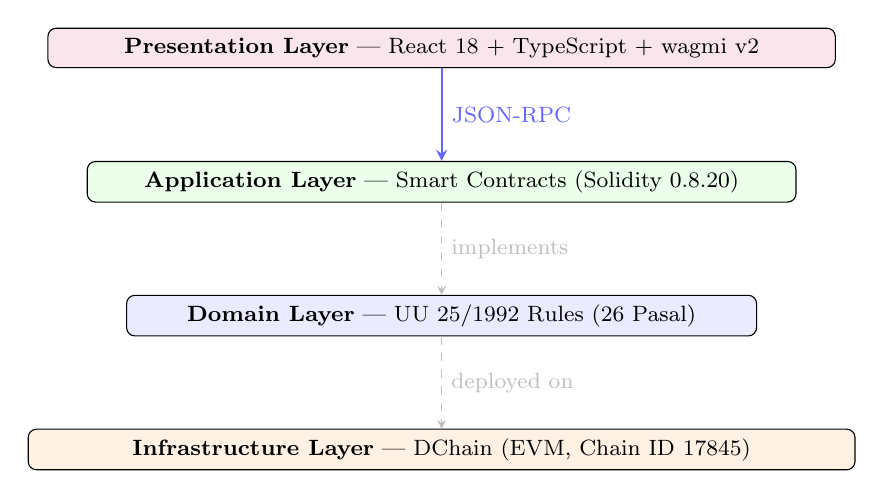
\begin{tikzpicture}[
    layer/.style={rectangle, draw, rounded corners=3pt, minimum width=8cm, minimum height=0.5cm, font=\footnotesize, align=center},
    arrow/.style={->, >=stealth, thick, blue!60},
    dep/.style={->, >=stealth, dashed, gray!50},
]
\node[layer, fill=purple!10, minimum width=10cm] (fe) at (0,3.5) {\textbf{Presentation Layer} --- React 18 + TypeScript + wagmi v2};
\node[layer, fill=green!8, minimum width=9cm] (app) at (0,1.8) {\textbf{Application Layer} --- Smart Contracts (Solidity 0.8.20)};
\node[layer, fill=blue!8, minimum width=8cm] (domain) at (0,0.1) {\textbf{Domain Layer} --- UU 25/1992 Rules (26 Pasal)};
\node[layer, fill=orange!10, minimum width=10.5cm] (infra) at (0,-1.6) {\textbf{Infrastructure Layer} --- DChain (EVM, Chain ID 17845)};
\draw[arrow] (fe.south) -- (app.north) node[midway, right, font=\footnotesize] {JSON-RPC};
\draw[dep] (app.south) -- (domain.north) node[midway, right, font=\footnotesize] {implements};
\draw[dep] (domain.south) -- (infra.north) node[midway, right, font=\footnotesize] {deployed on};
\end{tikzpicture}
\caption{Arsitektur \textit{Clean Architecture} Sistem Lakomi}
\label{fig:clean-architecture}
\end{figure}

Arsitektur ini mengikuti prinsip \textit{dependency inversion}: lapisan yang lebih tinggi bergantung pada abstraksi yang didefinisikan oleh lapisan di bawahnya, bukan sebaliknya. \textit{Domain Layer} (aturan UU 25/1992) adalah inti sistem yang tidak bergantung pada teknologi spesifik---perubahan pada infrastruktur blockchain (misalnya migrasi dari DChain ke platform EVM lain) tidak memerlukan perubahan pada aturan kepatuhan. \textit{Application Layer} (smart contract) mengimplementasikan aturan domain dalam bentuk kode yang dapat dieksekusi. \textit{Infrastructure Layer} menyediakan lingkungan eksekusi dan penyimpanan. \textit{Presentation Layer} menyediakan antarmuka pengguna yang berkomunikasi dengan \textit{Application Layer} melalui JSON-RPC.

Pemisahan yang ketat antara \textit{Domain Layer} (aturan hukum) dan \textit{Application Layer} (implementasi kode) adalah kontribusi arsitektural utama Lakomi: perubahan regulasi dapat diakomodasi melalui pembaruan \textit{smart contract} tanpa mengubah infrastruktur, sementara perubahan infrastruktur blockchain tidak memengaruhi aturan kepatuhan yang telah dikodekan.




